\section{Failure Analysis and Yield Improvement}

\subsection{Initial Observation}
The first production lots showed $\sim$65\% yield. Wafer test was dominated by \textbf{Pause Refresh Fail (Bin5)}. Defects appeared as uniformly scattered single-bit errors across the wafer (weak clustering, no edge/line signature). Storage-node capacitance met spec; SEM cross-sections at failed cells revealed no structural anomaly. Other CDs/films/electricals were within spec.

\begin{figure}[t]
  \centering
  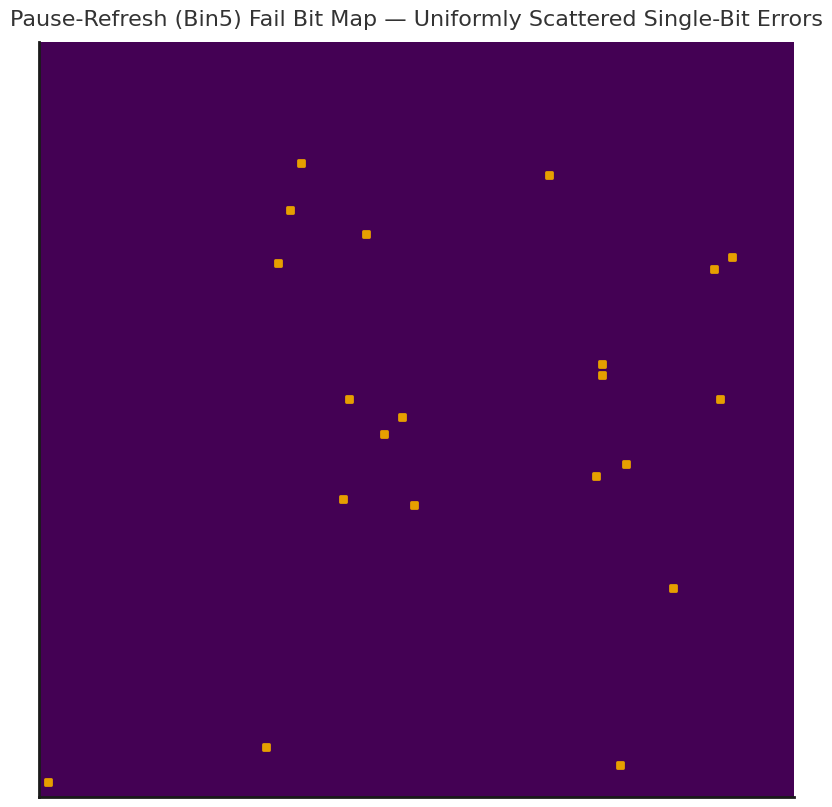
\includegraphics[width=\columnwidth]{fail_bitmap_bin5}
  \caption{Typical fail bit map under pause-refresh test (Bin5).
  Uniformly scattered single-bit errors are observed without edge/line signatures.}
  \label{fig:fail_bitmap}
\end{figure}

\subsection{Hypothesis (Failure Model)}
Directly measurable leakages were normal, suggesting a subtle leakage path. We hypothesized increased leakage at the \textbf{storage-node contact $n^+/p^-$ junction}. After gate etch, a remnant gate oxide on S/D active is repeatedly exposed to resist-stripping \emph{ashing} during multiple LDD steps. Cumulative plasma damage makes the oxide locally porous and can extend damage into the diffusion, creating minute leakage paths. This explains random single-bit distribution without visible structural defects.

% === Fig.2 Storage-node contact n+/p- leakage (pure TikZ, minimal IEEE style) ===
% --- 前置き(main.tex のプリアンブルに一度だけ)---
\usepackage{tikz}
\usetikzlibrary{arrows.meta,decorations.pathmorphing}

% --- 図本体(sections/results.tex などに)---
\begin{figure}[t]
  \centering
  \begin{tikzpicture}[x=5cm,y=3.3cm, line cap=round, line join=round]
    % 色とスタイル
    \definecolor{metgray}{RGB}{120,120,120}
    \tikzset{
      metal/.style={fill=metgray!20,draw=metgray,thick},
      poly/.style={fill=black!15,draw=black,thick},
      oxide/.style={fill=orange!10,draw=orange!60!black,thick},
      silicon/.style={fill=brown!10,draw=brown!60!black,thick},
      anno/.style={font=\scriptsize},
      leak/.style={very thick, dashed, -{Latex[length=2mm]}}
    }

    % 版面基準
    \def\xWL{0.10}   % WL の左端
    \def\wWL{0.18}   % WL 幅
    \def\xSN{0.36}   % SNコンタクト中心
    \def\xLOC{0.62}  % LOCOS 島の中心

    % 表面(ILD上面を灰、Si表面はy=0)
    \draw[black!40,thick] (0,0.68) -- (1.02,0.68) node[anno, right]{\small ILD};
    % フィールド酸化膜(LOCOS の「盛り上がり」)
    \draw[oxide] (\xLOC-0.14,0.00) .. controls (\xLOC-0.05,0.13) and (\xLOC+0.05,0.13) .. (\xLOC+0.14,0.00)
                 -- (\xLOC+0.14,-0.20) -- (\xLOC-0.14,-0.20) -- cycle;
    \node[anno] at (\xLOC+0.18,0.10) {LOCOS};

    % シリコン基板(p-)
    \draw[silicon] (0,-0.20) rectangle (1.02,-0.60);
    \node[anno] at (0.08,-0.52) {$p^{-}$~substrate};

    % n+ 拡散(WL 右側~LOCOS 手前)
    \draw[fill=cyan!15, draw=cyan!50!black, thick]
      (\xWL+\wWL+0.02,-0.02) rectangle (\xLOC-0.06,-0.20);
    \node[anno] at (0.44,-0.17) {$n^{+}$};

    % ワードライン(ポリシリコンゲート)
    \draw[poly] (\xWL,0.12) rectangle (\xWL+\wWL,0.35);
    \node[anno] at (\xWL+0.09,0.40) {WL};
    % ゲート下のチャネル表現(点線)
    \draw[densely dashed,black!60] (\xWL,0.12) -- (\xWL+\wWL,0.12);

    % ストレージノード(上部金属/電極)と縦コンタクト
    \draw[metal] (\xSN-0.06,0.62) rectangle (\xSN+0.06,0.68+0.10);
    \node[anno] at (\xSN,0.86) {SN};
    % ビア/コンタクトプラグ(縦)
    \draw[metal] (\xSN-0.018,0.12) rectangle (\xSN+0.018,0.68);

    % SN コンタークトの着地点(n+ 上)
    \draw[black,thick] (\xSN-0.06,0.12) -- (\xSN+0.06,0.12);
    \node[anno, anchor=west] at (\xSN+0.07,0.28) {storage-node contact};

    % 接触端近傍ダメージ(灰色斜線の小領域)
    \path let \p1 = (\xSN+0.06,0.12) in
      node[fill=metgray!30, draw=metgray, very thin, minimum width=10pt, minimum height=8pt, rotate=0]
      (damage) at (\xSN+0.085,0.06) {};

    \node[anno, anchor=west] at (\xSN+0.11,0.00) {plasma/LDD-induced damage};
    \node[anno, anchor=east] at (\xSN-0.10,-0.01) {junction leakage increase};

    % リーク経路(接触端→基板へ)
    \draw[leak] (\xSN+0.06,0.12) to[out=-75,in=75] (\xSN+0.04,-0.10)
                to[out=-105,in=80] (\xSN+0.02,-0.36);
    \node[anno, anchor=west] at (\xSN+0.08,0.16) {leakage path};

    % 目印(右上に LDD)
    \node[anno] at (0.97,0.78) {LDD};

  \end{tikzpicture}
  \caption{Storage-node contact ($n^+/p^-$) leakage consistent with the sketch:
  WL--$n^+$--LOCOS layout, SN contact landing on $n^+$, damage near the contact
  edge increases junction leakage and forms a leakage path.}
  \label{fig:storage_contact_tikz}
\end{figure}

\subsection{Countermeasures}
\begin{itemize}
  \item \textbf{Process}: Replace resist stripping in LDD steps from plasma ashing to \textbf{wet stripping (sulfuric-based)} to eliminate plasma damage. 
  \item \textbf{Integration hygiene}: Confirm downstream photo cleanliness and avoid residue risks with the wet strip.
\end{itemize}

\subsection{Effectiveness}
Yield improved from $\sim$65\% to \textbf{$\sim$80\%}. Uniformly scattered single-bit fails decreased markedly. Burn-in and retention/reliability passed; the final recipe was fixed for volume production.

% === Yield-by-lot (step improvement at countermeasure) ===
\begin{figure}[t]
\centering
\pgfplotstableread[col sep=comma]{data/yield_lot.csv}\yieldtbl
\begin{tikzpicture}
\begin{axis}[
  width=\columnwidth, height=0.58\columnwidth,
  xlabel={Lot ID}, ylabel={Yield [\%]},
  ymin=50, ymax=95,
  xmin=0.5, xmax=12.5,
  grid=both,
  xtick=data,
  xticklabels from table={\yieldtbl}{lot},
  xticklabel style={rotate=45, anchor=east},
]
  % データ描画
  \addplot+[mark=*] table[x expr=\coordindex+1, y=yield]{\yieldtbl};

  % 対策境界: lot04とlot05の間
  \draw[dashed] (axis cs:4.5,50) -- (axis cs:4.5,95);
  \node[anchor=west, font=\footnotesize] at (axis cs:4.55,92)
    {Countermeasure};
\end{axis}
\end{tikzpicture}
\caption{Yield step improvement at the countermeasure boundary
between \texttt{lot04} and \texttt{lot05}. Yield jumps from $\sim$62--63\% 
(lot01--lot04) to $\sim$82--84\% (lot05 onward) after changing 
LDD resist stripping from ashing to wet stripping.}
\label{fig:yield}
\end{figure}
